
Les signaux originales sont en stéréo, il faut les moyenner pour retrouver dans le cadre du cours.
fig.\ref{Fig.sub.1} est le signal avant moyenner, fig.\ref{Fig.sub.2} est le signal après moyenner.
\begin{figure}[htb]
\subfigure[Exemple de signal audio original]{
\label{Fig.sub.1}
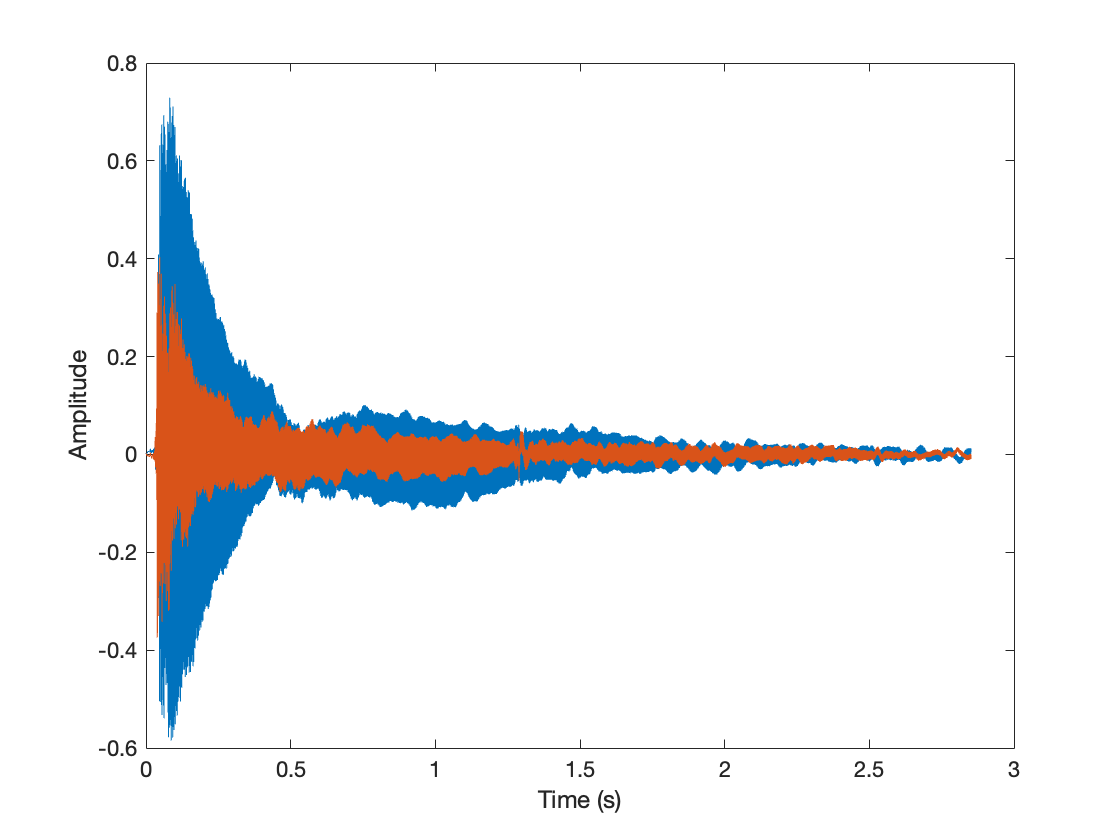
\includegraphics[width = 0.45\textwidth]{signal_before_mean.png}
}
\subfigure[Exemple de signal après moyenner]{
\label{Fig.sub.2}
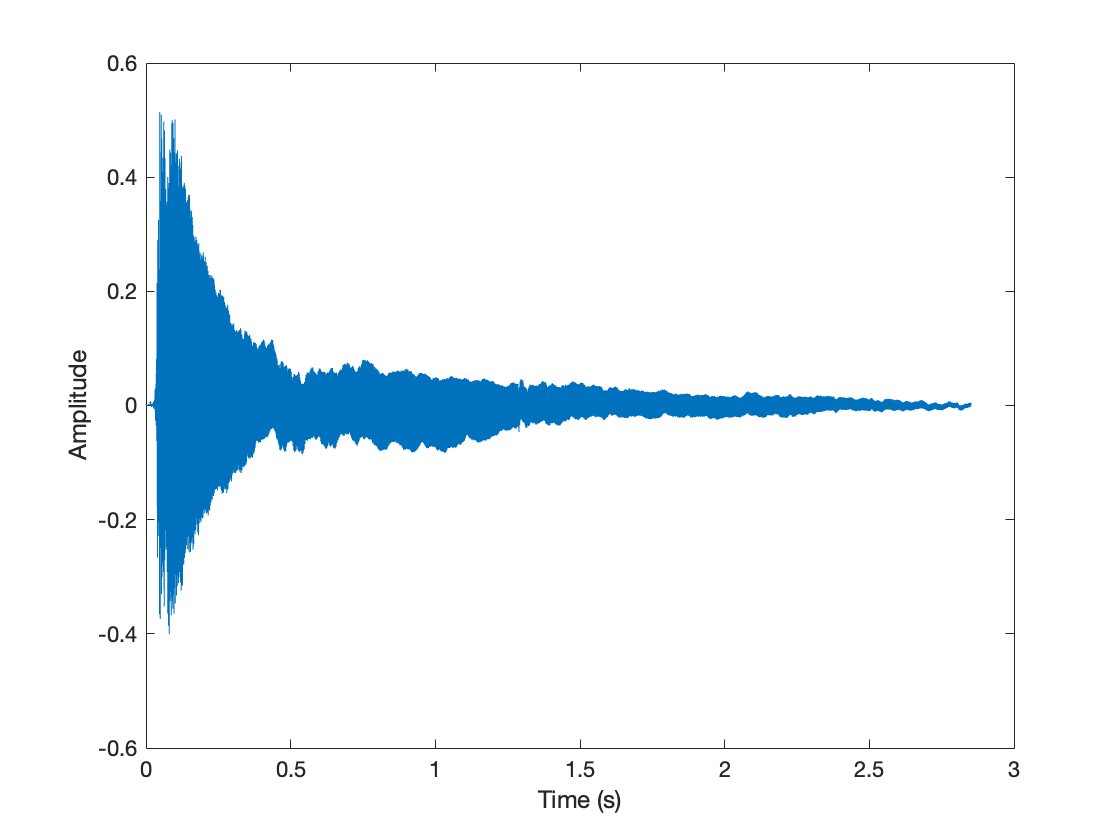
\includegraphics[width = 0.45\textwidth]{signal_after_mean.png}
}
\caption{Exemple de signal}
\label{Fig.main}
    % ici c'est le problem de overleaf que l'image ne marche pas
\end{figure}
